\documentclass[usenames, aspectratio=169]{beamer}

\usepackage{amsmath}
\usepackage{braket}
\usepackage{amsfonts}
\usepackage{tikz}
\usepackage{tikzpeople}
\usepackage{adjustbox}
\usepackage{subcaption}
\usepackage{svg}
\usepackage{graphicx}
\usepackage{media9}
\usepackage{float}
\usetikzlibrary{calc}
\usepackage{array}
\usepackage{efbox,graphicx}
\usepackage[normalem]{ulem}
\usepackage{verbatim}
\usepackage{ragged2e}
\usepackage{array}
\efboxsetup{linecolor=Green,linewidth=1.5pt, margin=0pt}

\usetikzlibrary{decorations.pathreplacing}

\newcommand\MemoryLayout[1]{
  \begin{tikzpicture}[scale=0.15]
    \draw[thick](0,0)--++(0,3)node[above]{$0$};
    \foreach \pt/\col/\lab [remember=\pt as \tp (initially 0)] in {#1} {
      \foreach \a [parse=true] in {\tp,...,\pt-1} {
        \draw[fill=\col](-\a, 0) rectangle ++(-1,2);
      }
      \draw[thick](-\pt,0)--++(0,3)node[above]{$\pt$};
      \if\lab\relax\relax\else
        \draw[thick,decorate, decoration={amplitude=1mm}]
        (-\tp,-0.2)--node[below=1mm]{\lab} (-\pt,-0.2);
      \fi
    }
  \end{tikzpicture}
}


\newcommand{\pslsq}[4]{
\begin{frame}
    \frametitle{#1} 
    \includegraphics[width=.7\linewidth]{#3}
    #4  
  \end{frame}
}

\newcommand{\psls}[4]{
  \begin{frame}
    \frametitle{#1} 
    \begin{columns}[t]
      \begin{column}{.48\textwidth}
        #4
      \end{column}
      \begin{column}{.52\textwidth}
        \adjincludegraphics[width=.98\linewidth, valign=t]{#3}
      \end{column} 
    \end{columns}
  \end{frame}
}
\usepackage{sagetex}
%\usepackage{libertine}
%\usepackage{emerald}
%\usepackage[T1]{fontenc}

\usetheme[progressbar=frametitle]{metropolis}
%\usetheme{EastLansing}
\title[Understanding Quantumness And Testability.] % (optional, only for long titles)
{Understanding Quantumness And Testability.}

\subtitle{  }
\author[D.~Ponarovsky] % (optional, for multiple authors)
	{D.~Ponarovsky\inst{1}}

\institute[HUJI] % (optional)
{  Faculty of Computer Science\newline
  Hebrew University of Jerusalem
}
\date[2023] % (optional)
{Master-Exam-Huji.}
\subject{Understanding Quantumness And Testability.}

\begin{document}
\input{sageutil.py}
\begin{frame}
  \maketitle
\end{frame}
%\pslsq{Today.}{0.3}{controller.png}{}
%\pslsq{Today.}{0.5}{controller-2-out.png}{}

\begin{frame}
  \frametitle{ Today. }
  \begin{itemize}
    \item<1-> Brif Review of Coding. 
    \item<2-> Quantum Error Correction Codes.
    \item<3->Good Classical Locally Testabile Codes and Good Qauntum LDPC.
  \end{itemize} 
\end{frame}


\begin{frame}
  \frametitle{Introduction.}
  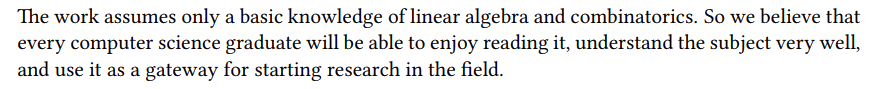
\includegraphics[width=.7\linewidth]{./Assumption-out.png}
\end{frame}



\begin{frame}
  \frametitle{ Coding. }
  \begin{center}
  
\begin{tikzpicture}
    \node[name=b, bob,monitor,minimum size=1cm,xshift=-7.2cm]{};
    \node[name= a, alice,monitor, mirrored,minimum size=1cm]{};
    \node (C) at (-3,0) {C};
    \draw[ -> ] (b.mouth) + (1,0) to (C)  ; 
  \end{tikzpicture}
\end{center}
\end{frame}

\begin{frame}
  \frametitle{ Coding. }
  Can we come up with a code that tolerates $*$ bits flip? 
\end{frame} 

\begin{frame}
  \frametitle{ Coding. }
\end{frame} 

\begin{frame}
  \frametitle{ Quantum Error Correction Codes. }
\end{frame} 

\begin{frame}
  \frametitle{ Coding. }
\end{frame} 

\begin{frame}
  \frametitle{ Coding. }
\end{frame} 

\begin{frame}
  \frametitle{ Coding. }
\end{frame} 


\psls{BUS.}{0.3}{./Peterson-out.png}{ 
  \begin{itemize}[<+->]
    \item  A BUS is a communication pathway that transfers data between different components of a computer.
    \item  Buses connect IO devices such as keyboards, monitors, and printers to the computer's central processing unit (CPU).
    \item  Buses provide a standardized way for different components to exchange data with each other, simplifying device connection and ensuring compatibility.
\end{itemize}
}



\end{document}
